% Teilauswertung 2
\newpage
\section{Dunkelfeldspektroskopie einer Nanorodprobe}
\label{sec:nanorods}

\begin{center}
    \captionsetup{type = figure}
    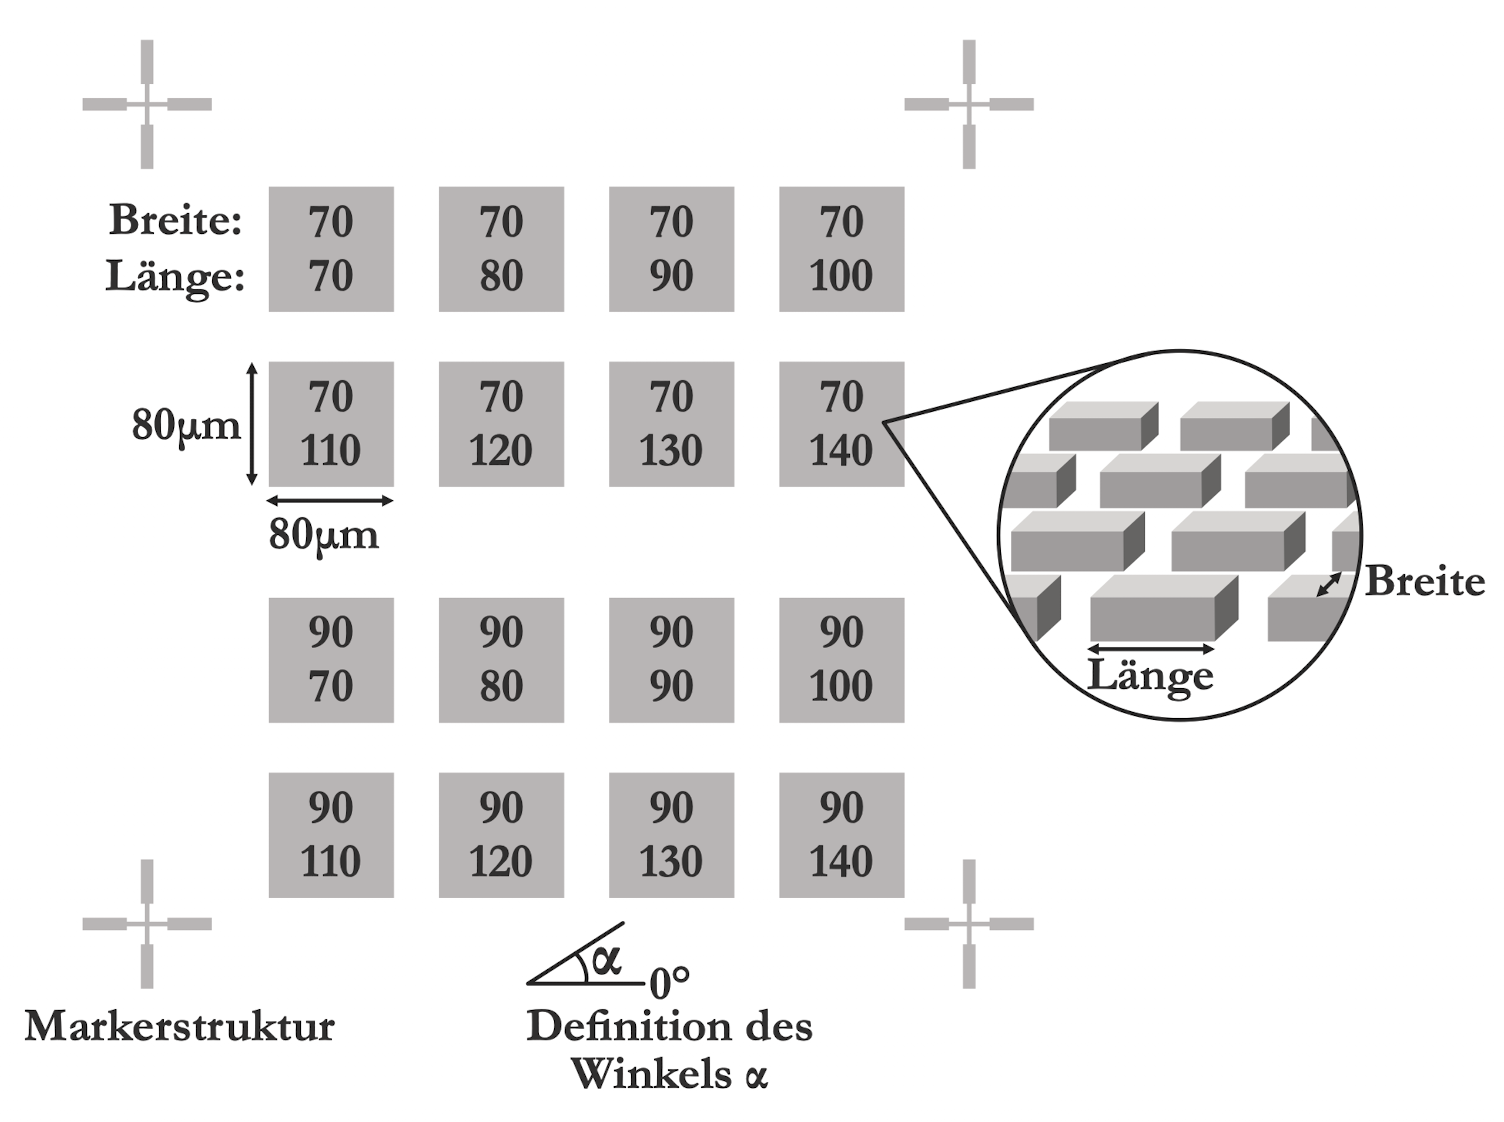
\includegraphics[width = \textwidth]{Bilder/Nanorods.png}
    \captionof{figure}{
        Übersichtsplan der verwendeten Probe. Die gesamte Probenstruktur befindet sich mehrmals auf einem Glassubstrat. Die Struktur selbst besteht aus Markern und 16 Feldern, die jeweils tausende Nanorod gleicher Dimensionen enthalten. Die Breite und Länge der Partikel in Nanometern sind auf den Feldern eingetragen. Das Inset zeigt die Vergrößerung eines einzelnen Probenfelds, wodurch die Orientierung der langen Achse der Rods und die Definition von Breite und Länge erkennbar ist. Der Winkel $\alpha$ ist unter dem Übersichtsplan definiert. Eine Polarisation von $\alpha = 0^\circ$ führt damit zu einer Anregung entlang der langen Achse der Rods. \cite{Anleitung}
    }
    \label{fig:nanorods}
\end{center}

In diesem Versuchsteil wurden mehrere Struktuten mit unterschiedlicher Nanorods (bestehend aus Silber) mit einer Breite von 70\,nm und 90\,nm und variabler Länge $L$ untersucht. Abbildung \ref{fig:nanorods} zeigt hierbei den Übersichtsplan der Probe, mit dem Parameter der Rods in den einzelnenFelder. Jedes Feld hat eine Größe von 80$\times$80\,$\mu$m und beinhaltet tausende identische Nanorods, womit das Streuspektrim aller Rods auf einem Feld gemessen werden kann. Der Winkel $\alpha$ gibt folgenden die Richtung der Polarisation an, wobei $\alpha = 0^\circ$ die Länge der Rods anregt und $\alpha = 90^\circ$ die Breite der Rods. \cite{Anleitung}

Es wurden einerseites die Spektren der Nanorods mit Intensität $I_\mathrm{N}$ als auch ein Dunkelspektrum $I_\mathrm{D}$ und ein Referenzspektrum $I_\mathrm{R}$ am Anfang und am Ende der Messung aufgenommen. Da in beiden Messungen das Dunkelspektrum mitgemessen wurde, wird dieses in der weiteren Rechnung nicht mehr beachtet (siehe auch Kapitel \ref{sub:korrigiertesSignal}). Um ein korrigieres Dunkelfeldspektrum $I_\mathrm{C}$ zu erhalten wird folgende Formel angewendet
\begin{gather}
    I_\mathrm{C} = \frac{I_\mathrm{N}}{\langle I_\mathrm{R} \rangle} ~,
\end{gather}
wobei $\langle I_\mathrm{R} \rangle$ der Mittelwert zwischen dem Referenzspektrum am Anfang und am Ende der Messung ist. Das korrigierte Dunkelfeldspektrum $I_\mathrm{C}$ (Einheit a.u. = arb. units) wurde in Abb. \ref{fig:spektrum} in Abhängigkeit der Wellenlänge $\lambda$ (Einheit nm) dargestellt. Dabei lässt sich für unpolarisiertes und polarisiertes Licht ($\alpha = 0^\circ$) erkennen, dass für zunehmende Rodlänge die Intensität $I_\mathrm{C}$ abnimmt. Für $\alpha = 90^\circ$ Polarisation ist dieser Effekt nur bei einer Rodbreite von 70\,nm zu erkennen, wobei hier zwei Maxima beobachtet werden können, welche selbst konstant sind für gewisse Rodlängen. Für eine Rodbreite von 90\,nm ist die Intensität unabhängig von der Rodlänge. Da erwartet wurde, dass sich die Intensität für eine Polarisation von $\alpha = 90^\circ$ nicht ändern sollte, lässt sich vermuten, dass bei der Messung von der Rodbreite 70\,nm ein Messfehler enstanden ist. 
\bigskip
Im nächsten Schritt wird durch einen Gauss-Fit die Maxima der Dunkelfeldspektren bestimmt. Die berechenten Werte können in Tabelle \ref{tab:nanorods} gefunden werden.
\newpage
\begin{sidewaysfigure}
    \centering
    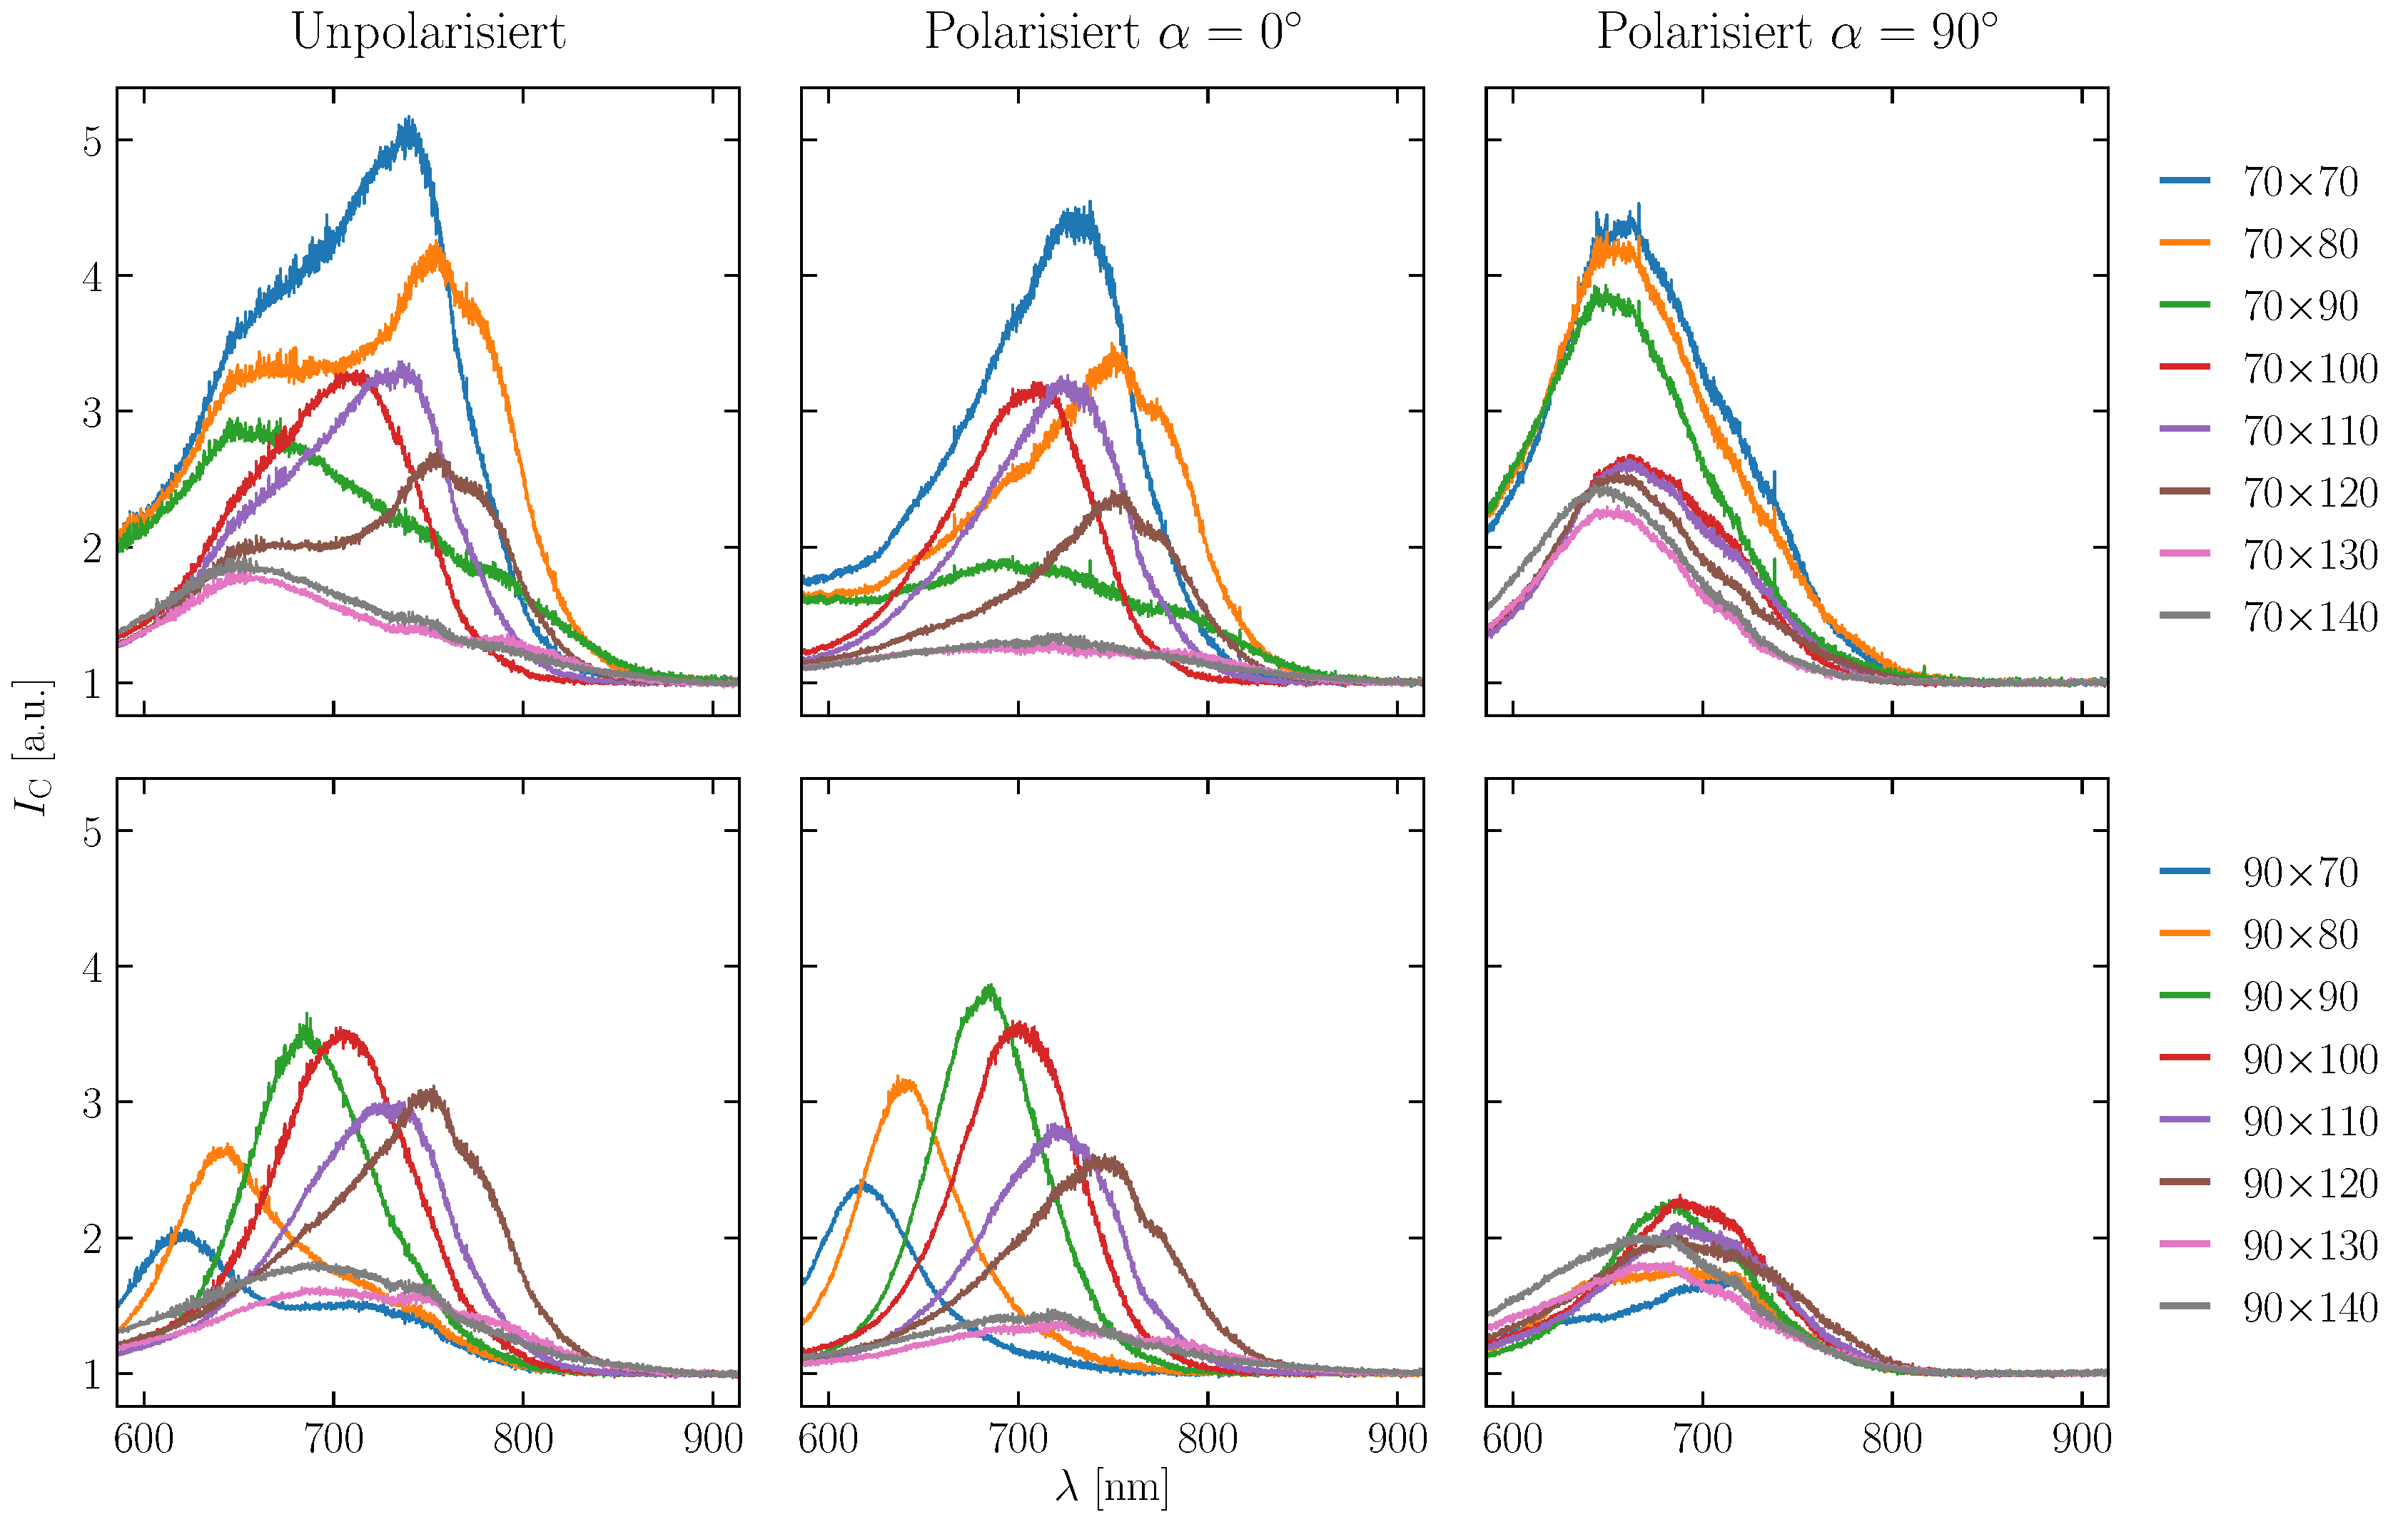
\includegraphics[width = \textheight]{Bilder/Auswertung/3.2/Spektren_Gruppe2.pdf}
    \caption{Korrigiertes Spektrum der Nanorodproben mit unpolarisierten und polarisierten ($\alpha = 0^\circ~;~90^\circ$) Lichtquelle. Die Rodlänge und die Rodbreite in Nanometer wurde mit Nomenklatur Rodbreite$\times$Rodlänge dargestellt}
    \label{fig:spektrum}
\end{sidewaysfigure}

\begin{center}
    \captionsetup{type = table}
    \begin{tabular}{r | c c c}
        $L$/nm & $\tilde{\lambda}^\mathrm{unpol}_{70}$/nm & $\tilde{\lambda}^\mathrm{\alpha = 0^\circ}_{70}$/nm & $\tilde{\lambda}^\mathrm{\alpha = 90^\circ}_{70}$/nm \\\hline
        70  & 704.97 $\pm$ 0.30 & 714.14 $\pm$ 0.25 & 664.06 $\pm$ 0.09 \\
        80  & 711.90 $\pm$ 0.45 & 731.00 $\pm$ 0.35 & 659.14 $\pm$ 0.10 \\
        90  & 670.03 $\pm$ 0.24 & 686.91 $\pm$ 0.28 & 651.89 $\pm$ 0.07 \\
        100 & 696.28 $\pm$ 0.15 & 700.19 $\pm$ 0.12 & 668.09 $\pm$ 0.06 \\
        110 & 711.12 $\pm$ 0.22 & 716.24 $\pm$ 0.15 & 668.05 $\pm$ 0.09 \\
        120 & 722.66 $\pm$ 0.47 & 741.14 $\pm$ 0.26 & 661.00 $\pm$ 0.11 \\
        130 & 669.37 $\pm$ 0.46 & 704.26 $\pm$ 0.34 & 653.20 $\pm$ 0.06 \\
        140 & 664.93 $\pm$ 0.26 & 704.78 $\pm$ 0.17 & 649.43 $\pm$ 0.05 \\
    \end{tabular}\\[0.5cm]
    \begin{tabular}{r | c c c}
        $L$/nm & $\tilde{\lambda}^\mathrm{unpol}_{90}$/nm & $\tilde{\lambda}^\mathrm{\alpha = 0^\circ}_{90}$/nm & $\tilde{\lambda}^\mathrm{\alpha = 90^\circ}_{90}$/nm \\\hline
        70  & 610.84 $\pm$ 1.64 & 619.92 $\pm$ 0.12 & 686.79 $\pm$ 0.29 \\
        80  & 653.88 $\pm$ 0.31 & 642.89 $\pm$ 0.09 & 678.25 $\pm$ 0.14 \\
        90  & 688.00 $\pm$ 0.06 & 683.02 $\pm$ 0.04 & 684.50 $\pm$ 0.06 \\
        100 & 703.85 $\pm$ 0.08 & 699.08 $\pm$ 0.07 & 690.43 $\pm$ 0.10 \\
        110 & 718.89 $\pm$ 0.13 & 716.34 $\pm$ 0.10 & 691.28 $\pm$ 0.09 \\
        120 & 735.59 $\pm$ 0.24 & 734.54 $\pm$ 0.15 & 687.75 $\pm$ 0.10 \\
        130 & 705.59 $\pm$ 0.14 & 714.76 $\pm$ 0.15 & 668.04 $\pm$ 0.09 \\
        140 & 689.79 $\pm$ 0.10 & 699.93 $\pm$ 0.15 & 664.27 $\pm$ 0.08 \\
    \end{tabular}
    \captionof{table}{
        Test
    }
    \label{tab:nanorods}
\end{center}